\section{Approach}
\label{sec:approach}
We propose a modular framework for transfer learning in reinforcement learning. 
The framework consists three modules: 
1) the \textbf{representation learner}, which constructs an abstract representation of the task environment;
2) the \textbf{policy learner}, which is RL learner operating based on the task abstraction created by the representation learner;
3) the \textbf{task environment}, which is the RL tasks to be solved by policy learner.

\subsection{Representation Learners}
The representation learner aims to construct an abstract and generalized representation of the task environment to facilitate later knowledge transfer.
Our framework includes several architectures as visualized in Figure \ref{fig:repr_learner}.
The architectures all include some lower-dimensional ``bottleneck'' layers, 
which are designed to enforce dimensionality reduction of the input.
Once learned, this intermediate latent space is expected to create a more compact and abstract representation of the original environment and serve as the basis of transfer learning. 

\begin{figure}[ht!]
	\centering
	\begin{subfigure}{0.45\columnwidth}
		\centering
		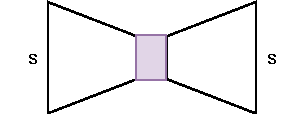
\includegraphics[width=\linewidth]{../img/very_simple_autoencoder.pdf}
		\caption{Simple autoencoder}
		\label{subfig:repr_learner_simple_autoencoder}
	\end{subfigure}%
	~ 
	\begin{subfigure}{0.45\columnwidth}
		\centering
		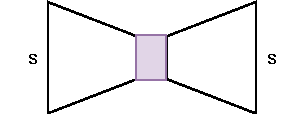
\includegraphics[width=\linewidth]{../img/very_simple_autoencoder.pdf}
		\caption{Variational autoencoder (add noise sign)}
		\label{subfig:repr_learner_vae}
	\end{subfigure}
	\begin{subfigure}{0.5\columnwidth}
		\centering
		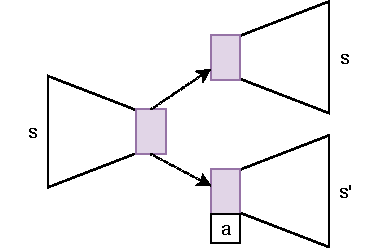
\includegraphics[width=\linewidth]{../img/janus.pdf}
		\caption{Janus}
		\label{subfig:repr_learner_janus}
	\end{subfigure}%
	~ 
	\begin{subfigure}{0.5\columnwidth}
		\centering
		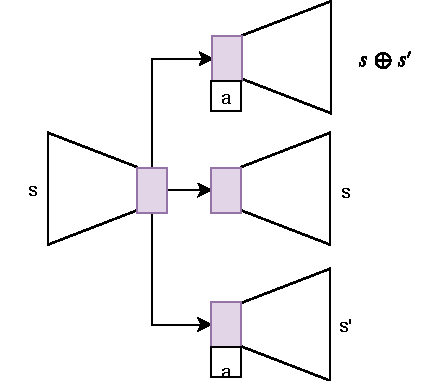
\includegraphics[width=\linewidth]{../img/cerberus.pdf}
		\caption{Cerberus}
		\label{subfig:repr_learner_cerberus}
	\end{subfigure}
	\caption{Network architectures of of representation learner, where $s$ and $s'$ indicate current and next state respectively, and $a$ indicates the action leading from $s$ to $s$. 
	The layers marked in purple are the latent representations to be used as the basis of later transfer learning. 
	The arrows indicate a straight copy from source to target.
	}
	\label{fig:repr_learner}
\end{figure}

\subsubsection{Simple and Variational Autoencoder}
The simplest representation learner is an autoencoder, which compresses and reconstructs the current state representation. 
Figure \ref{subfig:repr_learner_simple_autoencoder} illustrates the simple autoencoder, and \ref{subfig:repr_learner_vae} the variational autoencoder (VAE). 
%The VAE . 
However, one theoretical drawback is that
since the latent space only aims at compression, it is not necessarily a useful basis for transfer learning.
The upcoming architectures account for this.

\subsubsection{Janus}
To create more guidance in the construction of the latent space, we add another sub-network to capture the transition dynamics. 
As shown in Figure \ref{subfig:repr_learner_janus},
in addition to reconstructing the current state, we also append the action in latent space and seek to use this combination to predict the next state.
The hypothesized effect of this approach is that the latent representation can preserve the transition dynamics in the environment, and therefore is a more meaningful abstraction of the task.


\subsubsection{Cerberus}
Compared to Janus, the Cerberus architecture has one more output sub-network, which aims to construct the difference between the current and next state. 
By only predicting the differences, focus is placed on the change caused by the action taken.
This is especially useful when the changes between consecutive states are small relative to the entire state representation.
The network architecture is shown in Figure \ref{subfig:repr_learner_cerberus}.  

\subsection{Policy Learners}
Based on the latent space constructed by the representation learner, the policy learner is RL agent that .

\subsubsection{Table-based(?)}
Include or not?

\subsubsection{DQN}
\begin{itemize}
	\item avoid the exponential growth with state configurations
	\item DQN \citep{DQN} 
	\item with prioritized memory \citep{prioritized_memory} some memory is more important, depending on loss, give more prio to the ones that have major loss. Try to choose the ones causing more loss. 
\end{itemize}

\subsubsection{DDQN}
\begin{itemize}
	\item DDQN \citep{DDQN} also has prioritized memory 
	%Dueling DQN \citep{DuelingDQN}: state value, mix between q=learning and state action.
	\item DQN update policy every time. 
	\item continuously changing policy, estimate q-value changes every time.
	target network updated every 100 steps. prediction of q-values is fixed. otherwise there is ``more bias''?
\end{itemize}

\subsection{Integrating Representation and Policy Learners}
The interaction between the representation leaner and policy learner can occur in two ways, depending on the execution sequence of the two learning processes.

\begin{figure}[ht!]
	\centering
	\begin{subfigure}{0.45\columnwidth}
		\centering
		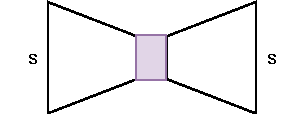
\includegraphics[width=\linewidth]{../img/very_simple_autoencoder.pdf}
		\caption{Simple autoencoder}
		\label{subfig:repr_learner_simple_autoencoder}
	\end{subfigure}%
	~ 
	\begin{subfigure}{0.45\columnwidth}
		\centering
		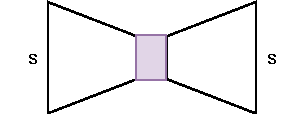
\includegraphics[width=\linewidth]{../img/very_simple_autoencoder.pdf}
		\caption{Variational autoencoder (add noise sign)}
		\label{subfig:repr_learner_vae}
	\end{subfigure}
	\begin{subfigure}{0.5\columnwidth}
		\centering
		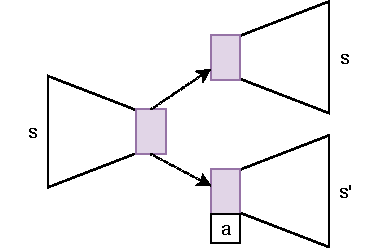
\includegraphics[width=\linewidth]{../img/janus.pdf}
		\caption{Janus}
		\label{subfig:repr_learner_janus}
	\end{subfigure}%
	~ 
	\begin{subfigure}{0.5\columnwidth}
		\centering
		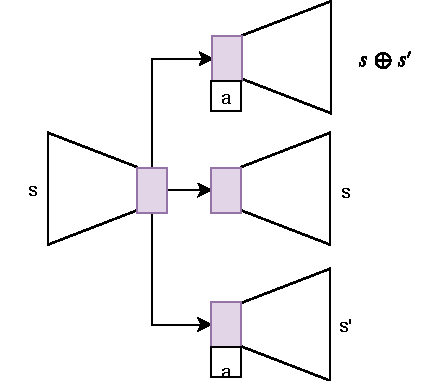
\includegraphics[width=\linewidth]{../img/cerberus.pdf}
		\caption{Cerberus}
		\label{subfig:repr_learner_cerberus}
	\end{subfigure}
	\caption{Network architectures of of representation learner, where $s$ and $s'$ indicate current and next state respectively, and $a$ indicates the action leading from $s$ to $s$. 
		The layers marked in purple are the latent representations to be used as the basis of later transfer learning. 
		The arrows indicate a straight copy from source to target.
	}
	\label{fig:approaches}
\end{figure}

\subsubsection{History Approach}
As the name indicates, the history approach first creates a collection of state, action and rewards by randomly exploring in the environment.
The representation learner is then trained based on the history.
Once learning completes, the policy learner is trained based on the encoding of the representation learner.
In this approach, the representation and policy learning are decoupled. 

\subsubsection{Parallel Approach}
In the parallel approach, the representation and policy learner are trained simultaneously.
observe the reward and new state. 
The policy learner is trained with loss from the observed reward.
The 



Encode using current encoder
Choose action and observe
%Use reward for policy loss
Use observation to calculate representation loss

